\vspace{-0.07in}
\section{Preliminaries}
\label{sec:setup}
%In this section, we present our problem setup. In total, we theoretically study the data reuse scaling behavior in linear regression problems.

% \paragraph{Notation.} 
% Throughout this work, we use letters for scalars and bold letters for vectors. We use \( \|\cdot\| \) to denote the \( \ell_2 \)-norm of vectors and the corresponding operator norm of matrices. For any given two sequences $\left\{A_n\right\}_{n=0}^{\infty}$ and $\left\{B_n\right\}_{n=0}^{\infty}$, we denote $A_n=O\left(B_n\right)$ if there exist some absolute constant $C_1>0$ and $N_1>0$ such that $\left|A_n\right| \leq C_1\left|B_n\right|$ for all $n \geq N_1$. Similarly, we denote $A_n=\Omega\left(B_n\right)$ if there exist $C_2>0$ and $N_2>0$ such that $\left|A_n\right| \geq C_2\left|B_n\right|$ for all $n>N_2$. We say $A_n=\Theta\left(B_n\right)$ if $A_n=O\left(B_n\right)$ and $A_n=\Omega\left(B_n\right)$ both holds. We say $A_n = o(B_n)$ (or $A_n \ll B_n$ or $B_n \gg A_n$) if for arbitrary positive constant $C_3 > 0$, there exists $N_3 > 0$ such that $|A_n| < C_3 |B_n|$ for all $n>N_3$. And we also use $A_n \approx B_n$ to denote $A_n = B_n + o(1)$. For two vectors \( \vu \) and \( \vv \) in a Hilbert space, we denote their inner product by \( \langle \vu, \vv \rangle \) or \( \vu^\top \vv \). For two matrices \( \mA \) and \( \mB \) of appropriate dimensions, we define their inner product as \( \langle \mA, \mB \rangle := \tr(\mA^\top \mB) \). Finally, \( \log(\cdot) \) refers to the logarithm with base $e$, where $e$ is the natural exponent.
% \haodong{add notations for big O notation}
\paragraph{Notations.}
%Throughout this work, we use letters for scalars and bold letters for vectors. 
We use \( \|\cdot\| \) to denote the \( \ell_2 \)-norm of vectors and the corresponding operator norm of matrices. 
For two sequences \((A_n)_{n=0}^\infty\) and \((B_n)_{n=0}^\infty\), we write 
\(A_n = O(B_n)\), or alternatively $A_n \lesssim  B_n$, $B_n = \Omega(A_n)$, $B_n \gtrsim A_n$, if there exist constants \(C>0, N>0\) such that \(|A_n|\leq C|B_n|\) for all \(n \geq N\). %We write $A_n = \Omega(B_n)$, or alternatively $A_n \gtrsim  B_n$, if $B_n = O(A_n)$. 
We write $A_n = \Theta(B_n)$, or alternatively $A_n \asymp  B_n$, if both $A_n = O(B_n)$ and $A_n = \Omega(B_n)$ hold.
Moreover, for some variable $n$, we write $A_n = o_n(B_n)$ if for every constant \(c>0\), there exists \(n_0>0\) such that \(|A_n| < c|B_n|\) for all \(n \geq n_0\). In this paper, when $n$ is clear from the context, we write $A_n = o(B_n)$ for short. Furthermore, we write $A_n = \omega(B_n)$ if $B_n = o(A_n)$. For matrices $\mA_1, \mA_2,\dots,\mA_n$, we use $\prod_{l=1}^n \mA_l$ to denote the product $\mA_1\mA_2\dots\mA_n$. We define $\|\boldsymbol{u}\|_{\mS} := \sqrt{\boldsymbol{u}^\top \mS\boldsymbol{u}}$ for any vector $\boldsymbol{u}$ and any positive semi-definite (PSD) matrix $\mS$.

%; and \(A_n \approx B_n\) if \(A_n = B_n + o(1)\). 
% For vectors \(\vu, \vv\) in a Hilbert space, we denote their inner product by \(\langle \vu, \vv \rangle\) or \(\vu^\top \vv\). 
% For matrices \(\mA, \mB\) of compatible dimensions, we define \(\langle \mA, \mB \rangle := \tr(\mA^\top \mB)\). 
% Finally, \(\log(\cdot)\) refers to the natural logarithm with base \(e\).

\paragraph{Linear Regression Problem.} We focus on a linear regression setup, where data point $(\vx,y) \in \mathbb{R}^{d}\times\mathbb{R}$ follows a joint distribution $\mathcal{D}$ and $\|\vx\|\leq D$ for some constant $D$. W.L.O.G., we assume that the covariance matrix of data input is diagonal, i.e., $\mH := \E[\vx\vx^\top] = \diag \left(\lambda_1, \lambda_2, \dots, \lambda_{d}\right) $, where $\lambda_1 \geq \lambda_2 \geq \dots \geq \lambda_{d}$. A direct corollary is that $\lambda_1 \leq D^2$. For a given data input $\vx$, the label $y$ is generated by $y:= \langle \vw^*, \vx \rangle + \xi$, where $\vw^* \in \mathbb{R}^{d}$ is the ground-truth weight and $\xi$ represents the independent random label noise with $\E[\xi] = 0$ and $\E[\xi^2] = \sigma^2$. We aim to train a linear model $f(\vx; \vw):=\langle \vw, \vx \rangle$ to predict the data label, where $\vw \in \mathbb{R}^{d}$ is the trainable parameter. We use MSE-loss $\ell(\vw; \vx, y):=\frac{1}{2}(f(\vx; \vw)-y)^2$ to measure the fitting error. Then, the population loss is defined as $\cL(\vw):= \E_{(\vx, y) \sim \cD}[\ell(\vw;\vx, y)]$. Further we define the excess risk $\cR(\vw) := \cL(\vw) - \frac{1}{2}\sigma^2$, which is the expected population loss minus the irreducible loss $\frac{1}{2}\sigma^2$.
%and the excess risk is defined as $\E_{\vw}\cR(\vw):=  \E_{\vw}\cL(\vw)- \frac{1}{2}\sigma^2$,

% \begin{figure}[t!]
%     \centering
%     \subfigure[$E(K,N)$ v.s.~$K$.%
%       \label{fig:ek-k}]{
%         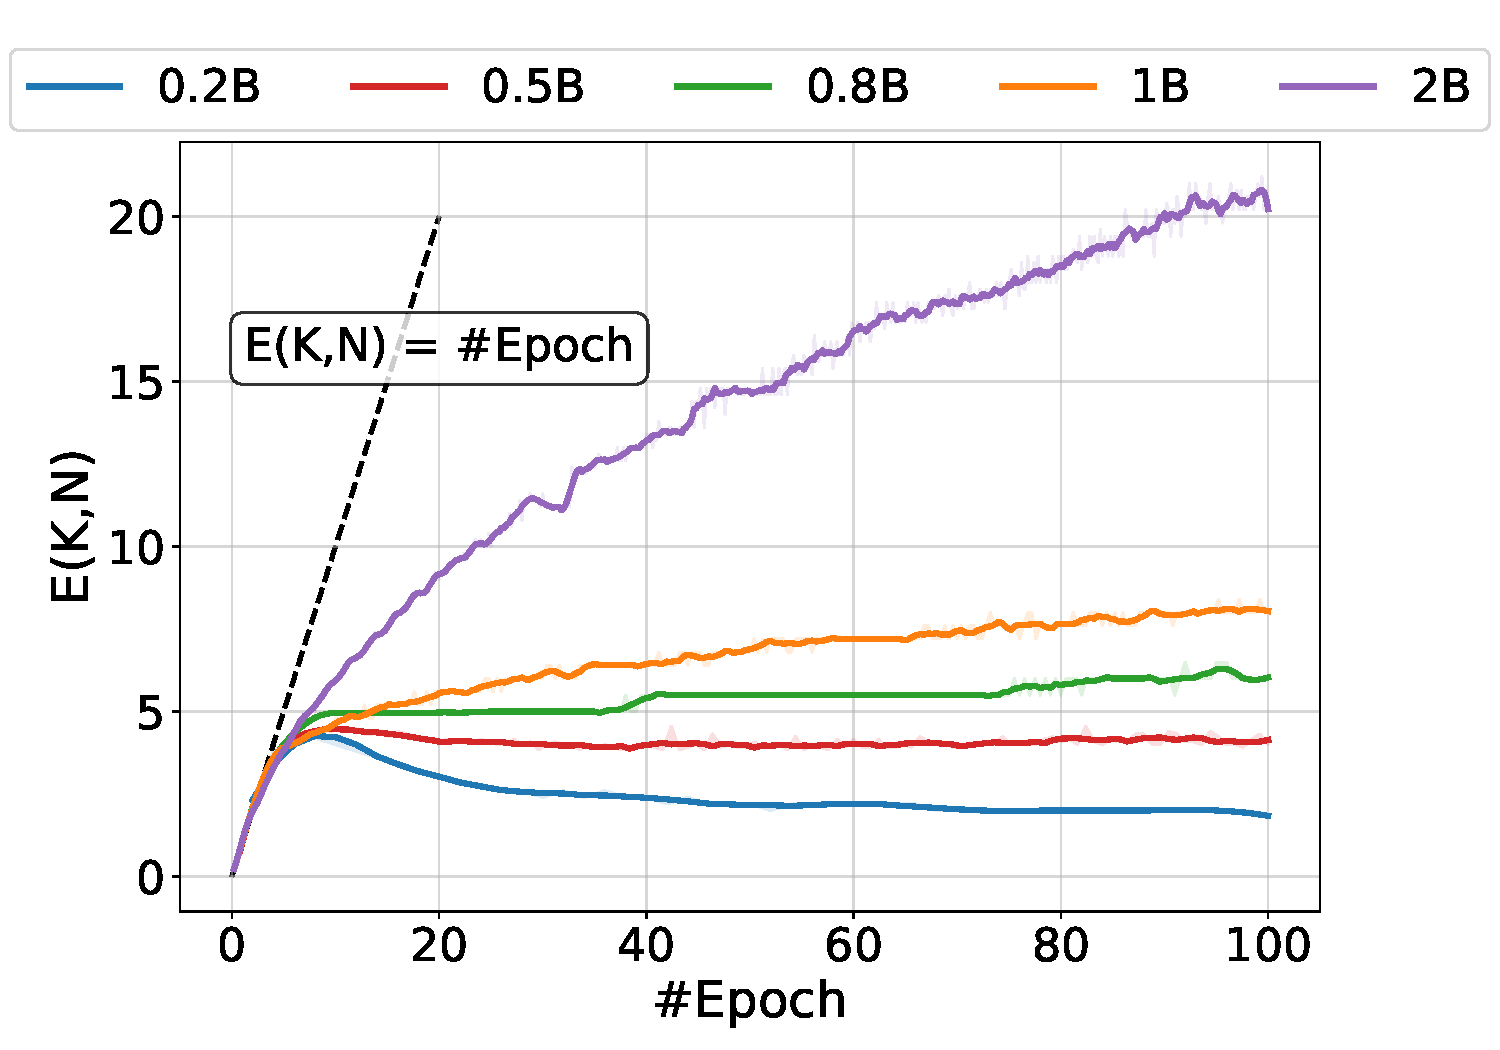
\includegraphics[width=0.48\linewidth]{figs/E_k_smoothed_shaded.pdf}
%     }\hfill
%     \subfigure[$E(K,N)$ v.s.~$N$.%
%       \label{fig:ek-data}]{
%         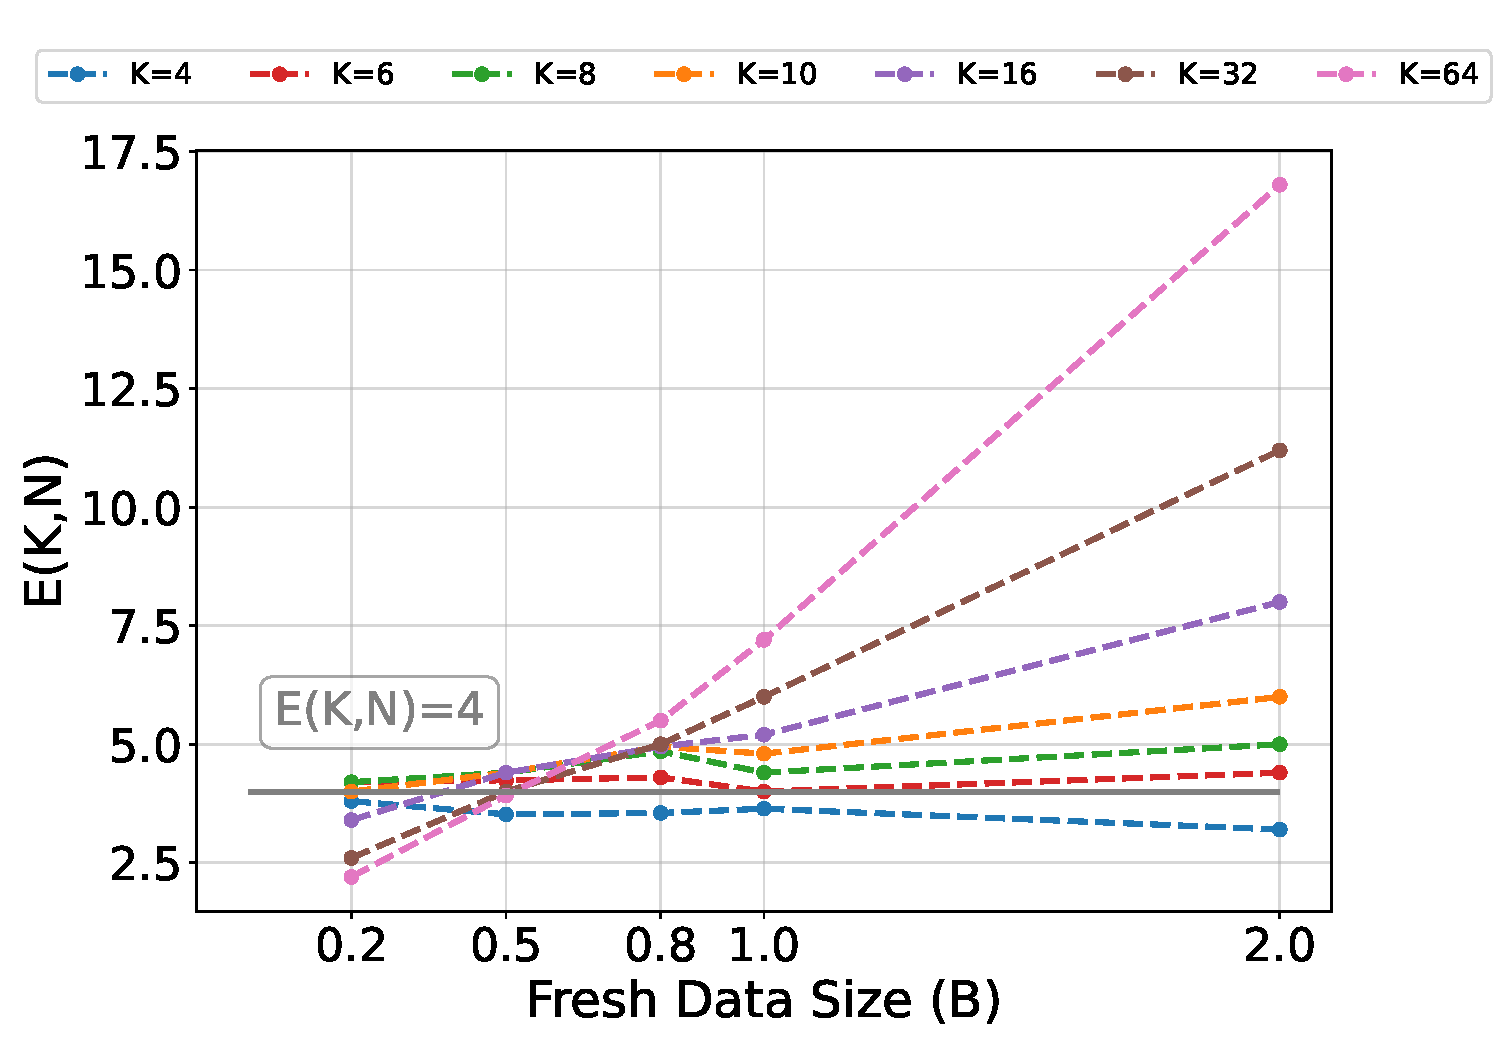
\includegraphics[width=0.48\linewidth]{figs/E_k_over_fresh_data_size.pdf}
%     }
%     \caption{In language model experiments, the effective reuse rate $E(K,N)$ behaves as follows:
%     (1) With $N$ fixed, $E(K,N)$ grows with $K$ before saturating at a value that increases with $N$;
%     (2) With $K$ fixed, $E(K,N)$ grows with $N$ and saturates at $K$.}
% \end{figure}

% \haodong{fix the definition of excess risk}
%Consider a linear regression problem with population loss $\cL(\vw) = \frac{1}{2} \E[(\langle \vw,\;\vx \rangle - y^*)^2]$, where $\vw \in \R^d$ represents the trainable parameter, $y^* = \langle \vw^*, \vx\rangle$, $\E\vx\vx^{\top}=\mH$, and $\vw^*$ is the ground truth.
\paragraph{Multi-Epoch SGD Training Algorithm.} Consider a finite training dataset with $N$ data points $\{(\vx_0,y_0),(\vx_1,y_1),\dots,(\vx_{N-1},y_{N-1})\}$, where the data points $(\vx_i, y_i)$ are i.i.d.~sampled from the distribution $\mathcal{D}$. We use $K$-epoch stochastic gradient descent (SGD) with random shuffling to minimize the loss function. And the initial parameter $\vw_0$ is set to $0$. Formally, we denote $K$ independent random permutations of $[N]$ by $\pi_1, \dots, \pi_K$. And we define $j_t := \pi_{k_t}(i_t)$, where $i_t := t \bmod N$, $k_t := \lfloor t / N \rfloor + 1$. Then we have the update rule for $K$-epoch SGD with $N$ data points
% \begin{align*}
%     \vw_{t+1} &= \vw_{t} - \eta \nabla_{\vw}\ell(\vw_t; \vx_{j_t}, y_{j_t}) \\
%     &=\left(\mI-\eta\vx_{j_t}\vx_{j_t}^{\top}\right)\vw_t+\eta\xi_{j_t}\vx_{j_t}.
% \end{align*}
\begin{equation}
    \vw_{t+1} = \vw_{t} - \eta \nabla_{\vw}\ell(\vw_t; \vx_{j_t}, y_{j_t}) =\left(\mI-\eta\vx_{j_t}\vx_{j_t}^{\top}\right)\vw_t+\eta\xi_{j_t}\vx_{j_t}. \nonumber
\end{equation}
Next, given a $K$-epoch SGD over $N$ data points, with learning rate $\eta$, we define $\cW_{K,N,\eta}$ to be the distribution of $\vw_{KN}$. The randomness within $\vw_{KN}$ comes from the random draw of the dataset, label noise $\xi$, and the shuffling in SGD. Based on this, we define the expected excess risk of a given $K$-epoch SGD over $N$ data points, with learning rate $\eta$ as $\bar{\cR}(K, N; \eta) := \E_{\vw \sim \cW_{K,N,\eta}}[\cR(\vw)]$. We assume $\eta \leq D^{-2}$ for training stability.

We also consider multi-epoch training under more practical training configurations, for example, using a class of polynomially decaying learning-rate schedules. See \Cref{app:discussion} for more details.
% \kaifengclaw{Typo/style: 'multi epoch' -> 'multi-epoch'; 'a polynomial decaying learning rate schedule class' can be simplified to 'a class of polynomially decaying learning-rate schedules'.}
% where $\eta$ is the learning rate, and $\pi_k$ denotes the permutation mapping in the $k$-th epoch that sends the i-th data to index $\pi_k(i)$. We assume $\eta < D^{-2}$ for training stability.
% \kaifeng{noise can cause oscillation too}

\begin{comment}
-----------

Given training time $t\in[(k-1)N, kN)$ for some $k\in\mathbb{N^*}$, we define $i_t:= t - (k-1)N \in [0, N-1]$.

$\vw_{k,i} $

$i_t = t \bmod N$

We define an alternative notation for $\vw_t$ as $\vw_{k, i+1}$, where $k$ represents the number of completed epochs and $i+1$ denotes the additional data points processed in the current epoch. Then the $t+1$-th iteration is given by
\begin{align*}
    \vw_{t+1} &= \vw_{t} - \eta \nabla_{\vw}\ell_{\vw_{t}}(\vx_{\pi_k(i)}, y_{\pi_k(i)}) \\
    &=\left(\mI-\eta\vx_{\pi_k(i)}\vx_{\pi_k(i)}^{\top}\right)\vw_t+\eta\xi_{\pi_k(i)}\vx_{\pi_k(i)},
\end{align*}
where $\eta$ is the learning rate, and $\pi_k$ denotes the permutation mapping in the $k$-th epoch that sends the i-th data to index $\pi_k(i)$. 
We assume $\eta < D^{-2}$ to avoid oscillation.\kaifeng{noise can cause oscillation too}


$\cW_{K,N}(\eta)$: the distribution of $\vw_{KN}$, where $\vw_{KN}$ is the weight at the last iteration of $K$-epoch SGD with data size $N$. The randomness comes from the random draw of the dataset and the shuffling in SGD

$\vw_{k,s} = \vw_{kN+s}$


With learning rate $\eta$, we denote the parameter updated by one-pass SGD at step $T$ by $\vw_T(\eta)$, and we the parameter updated by multi-epoch SGD at $k$-th epoch with dataset size $N$ is denoted by $\vw_{K,N}(\eta)$. When causing no confusion, we omit $(\eta)$ and denote them by $\vw_T$ and $\vw_{K,N}$ for short.
% from index $i$  to the corresponding index in the training dataset. 
\end{comment}

\paragraph{Comparing Performance under Optimal Learning Rate Regime.} %The learning rate plays a critical role in shaping the training dynamics of linear regression under SGD. Therefore, to enable a fair and meaningful comparison between one-pass and multi-epoch SGD, careful tuning of the learning rate is essential. 
To compare the performance of one-pass and multi-epoch SGD, we consider the settings where the learning rates for both methods are optimally tuned.
% tuned to the optimal.
% \kaifengclaw{Clarity: 'tuned to the optimal' sounds awkward; suggest 'optimally tuned' or 'tuned to their respective optima'.}
Formally, we introduce the notion of the \textit{optimal expected excess risk} of $K$-epoch SGD for $N$ samples as $\bar{\cR}^*(K, N):=\min_{\eta \in (0, \frac{1}{D^2}]}\{ \bar{\cR}(K, N; \eta) \}$. To calculate this value analytically, in the next section, we will show that we can get a learning rate choice that can approximately achieve the above optimal expected excess risk $\bar{\cR}^*(K, N)$ both for one-pass and multi-epoch SGD.
% \kaifengclaw{Typo/clarity: 'in math' -> 'analytically'; this sentence is long and repetitive ('we will show... we can get... can approximately achieve'). Consider splitting into two shorter sentences.}
Following our discussion in the introduction, we define the \textit{effective reuse rate} as follows:
\begin{definition}[Effective Reuse Rate]\label{def:E_K}
Given $K$-epoch SGD trained with $N$ fresh data samples, the effective reuse rate is defined as: $E(K,N) := \frac{1}{N}\min\{N' \ge 0: \bar{\cR}^*(1, N') \leq\bar{\cR}^*(K, N)\}$.
%%%$\kaifengclaw{Math-check: since $N'$ is a sample size, should the minimization domain be integers ($N'\in\mathbb{N}$)? If treated continuously for asymptotics, consider stating this explicitly to avoid ambiguity in derivations.}\kaifeng{no. it is clear that $N'$ is an integer.}
% \kaifengclaw{Consistency: earlier/later you use 'effective reuse rate'; here it says 'ratio'. Better keep one term consistently throughout.}
%\begin{equation}
%    E_{\eta, \eta'}(K,N) := \frac{1}{N}\min\{T' : \E[\cR(\vw_{T'}(\eta'))] \leq \E[\cR(\vw_{K,N}(\eta))]\}. \nonumber
%\end{equation}
% \begin{equation}
%     E_{\eta, \eta'}(K,N) := \frac{1}{N}\min\{T' : \bar{\cR}(1, T'; \eta') \leq \bar{\cR}(K, N; \eta)\}. \nonumber
% \end{equation}
% \begin{equation}
%     E(K,N) := \frac{1}{N}\min\{N' \ge 0: \bar{\cR}^*(1, N') \leq\bar{\cR}^*(K, N)\}. \nonumber
% \end{equation}
% \tingkai{Explanations}
% where $\bar{\cR}^*(K, N)$ denotes the optimal excess risk of $K$-epoch SGD trained with $N$ fresh data samples. Specifically $\bar{\cR}^*(1, N')$ denotes the optimal excess risk of one-pass SGD with steps $N'$.
\end{definition}

\vspace{-0.05in}
That is, the effective reuse rate measures how many times larger the dataset must grow under one-pass training to match the performance of $K$-epoch training, both under the optimal learning rate regime.


%This definition characterizes the equivalent number of epochs required for OP SGD with the optimal learning rate, corresponding to the optimal expected excess risk of ME SGD. This definition characterizes the effectiveness of scaling in data reusing regime.
%To study the scaling behavior of data reusing, 

%we first tune the learning rate of one-pass (OP) SGD to be as close to optimal as possible, thereby establishing a baseline for comparison. Subsequently, we design an approximately optimal learning rate for multi-epoch (ME) SGD and compare its performance with that of the other methods. However, precisely determining the optimal learning rate for both OP and ME SGD remains challenging. To address this, 

% \[
%     \bar{\cR}^*(K, N):=\min_{\eta \in (0, \frac{1}{D^2}]}\{ \bar{\cR}(K, N; \eta) \}.
% \]
%$\eta^* = \eta^*(K,N) = \arg\min_{\eta \in (0, \frac{1}{D^2})}\E\left[\cR\left(\vw_{K,N}(\eta)\right)\right]$. 

% optimal excess risk of $K$-epoch SGD for $N$ samples: $\bar{\cR}^*(K, N):=
% \min_{\eta \in (0, \frac{1}{D^2})}\{ \bar{\cR}(K, N; \eta) \}$.

%$\eta^*(K,N) \in \argmin_{\eta \in (0, \frac{1}{D^2})}\{ \bar{\cR}(K, N; \eta) \}$. We choose an arbitrary 

%\E\left[\cR\left(\vw_{K,N}(\eta^*)\right)\right]$.

% Also, we can denote that the minimal excess risk achieved by the optimal learning rate $\E[\cR^*(\vw_{K,N})] :=\E[\cR^*(\vw_{K,N}(\eta^*))]$. Then we show in the next section that we can get an alternative learning rate choice that can approximately achieve the minimal excess risk of the optimal learning rate $\eta^*$.
% \haodong{definition not even clear}
%maybe we don't need this def
% \begin{definition}[Optimal Learning Rate]\label{def:opt-lr}
%     We define the optimal learning rate with completed training epochs $K$ and dataset size $N$ as
%     \begin{align*}
%         \eta^* = \eta^*(T) = \arg\min_{\eta \in (0, \frac{1}{D^2})}\E\left[\cR\left(\vw_{K,N}(\eta)\right)\right].
%     \end{align*}
% \end{definition}
% Futher, we can denote that the minimal excess risk achieved by the optimal learning rate $\E[\cR^*(\vw_{K,N})] :=\E[\cR^*(\vw_{K,N}(\eta^*))]$.

% \begin{definition}[Approximate Expected Population Excess Risk]\label{def:A-loss}
%     We say that a function $\widehat{\cR}:\mathbb{N}\times\mathbb{R}\rightarrow\mathbb{R}$ is an approximate population excess risk at iteration $T$ within a range $[f(T), g(T)]$ for two functions $f(T), g(T) = o_T(1)$ that satisfies $\eta^* \in [f(T), g(T)]$, if $\E[\cR(\vw_T(\eta))] = \widehat{\cR}(T, \eta)(1+o_T(1))$ holds for all learning rates $\eta \in [f(T), g(T)]$. 
% \end{definition}

% Based on the above approximate population excess risk, we define the following approximately optimal learning rate.

% \begin{definition}[Approximately Optimal Learning Rate]\label{def:A-opt-lr}
% %     For a given total training time $T$, we define the approximately optimal learning rate set as follows:
% % \begin{equation}
% %     \Gamma_{T}:=\{\eta^*: \exists \text{ an approximate population excess risk }\widehat{\cR} \text{ s.t. } \eta^*\in \operatorname{\arg \min}_{\eta} \widehat{\cR}(T, \eta) \}. \nonumber
% % \end{equation}
% % \kairong{I guess here $\Gamma_T$ is actually $\Gamma_T(\widehat{\cR})$}

% % For the expected loss estimate $\E[\cL(\vw_T)] = \fakeE[\cL(\vw_T)](1 + o(1))$, then we define the set of asymptotic optimal learning rates $\Gamma_{A-opt}$ is the set  such that
% % \begin{align*}
% %     \Gamma_{A-opt} := \{\eta_*: \eta_* = \arg \min_{\eta} \fakeE[\cL(\vw_T)]\}.
% % \end{align*}
% \end{definition}
%\vspace{-0.75em}
%\paragraph{Effective Reuse Rate.}
% \haodong{I think we need one sentence more for the transition from the choice of learning rate to $E_K(K,N)$} 
%Now, we formally introduce the key concept in our paper as follows:
% \haodong{also we need some interpretation for this definition here}
%     Given $K$-epoch SGD with some learning rate $\eta_{\ME} = f(K,N)$, whose expected loss after $T=KN$ steps is denoted by $\E[\cL_{\ME}(\vw_{KN})]$ and one-pass SGD with learning rate $\eta_{\OP} = g(T')$, whose expected loss after $T'$ is denoted by $\E[\cL_{\OP}(\vw_{T'})]$, we define the effective number of epochs as
%     \begin{align*}
%         E_K = \frac{1}{N}\min\{T':\E[\cL_{\OP}(\vw_{T'})]  \le \E[\cL_{\ME}(\vw_{KN})]\},
% \end{align*}
% where $f(\cdot,\cdot):\R^+\times\R^+\to\R^+$, and $g(\cdot):\R^+\to\R^+$
